\section{Building Blocks}\label{building-blocks}

\subsection{Level 1 Main Scope and
Context}\label{level-1-main-scope-and-context}

The following diagram represents the main component in the framework
divided by four subsystems:

\begin{itemize}
\tightlist
\item
  Client Subsystem
\item
  Processing Subsystem
\item
  Storage Subsystem
\item
  UI Subsystem
\end{itemize}

\begin{figure}[!h]
	\centering
	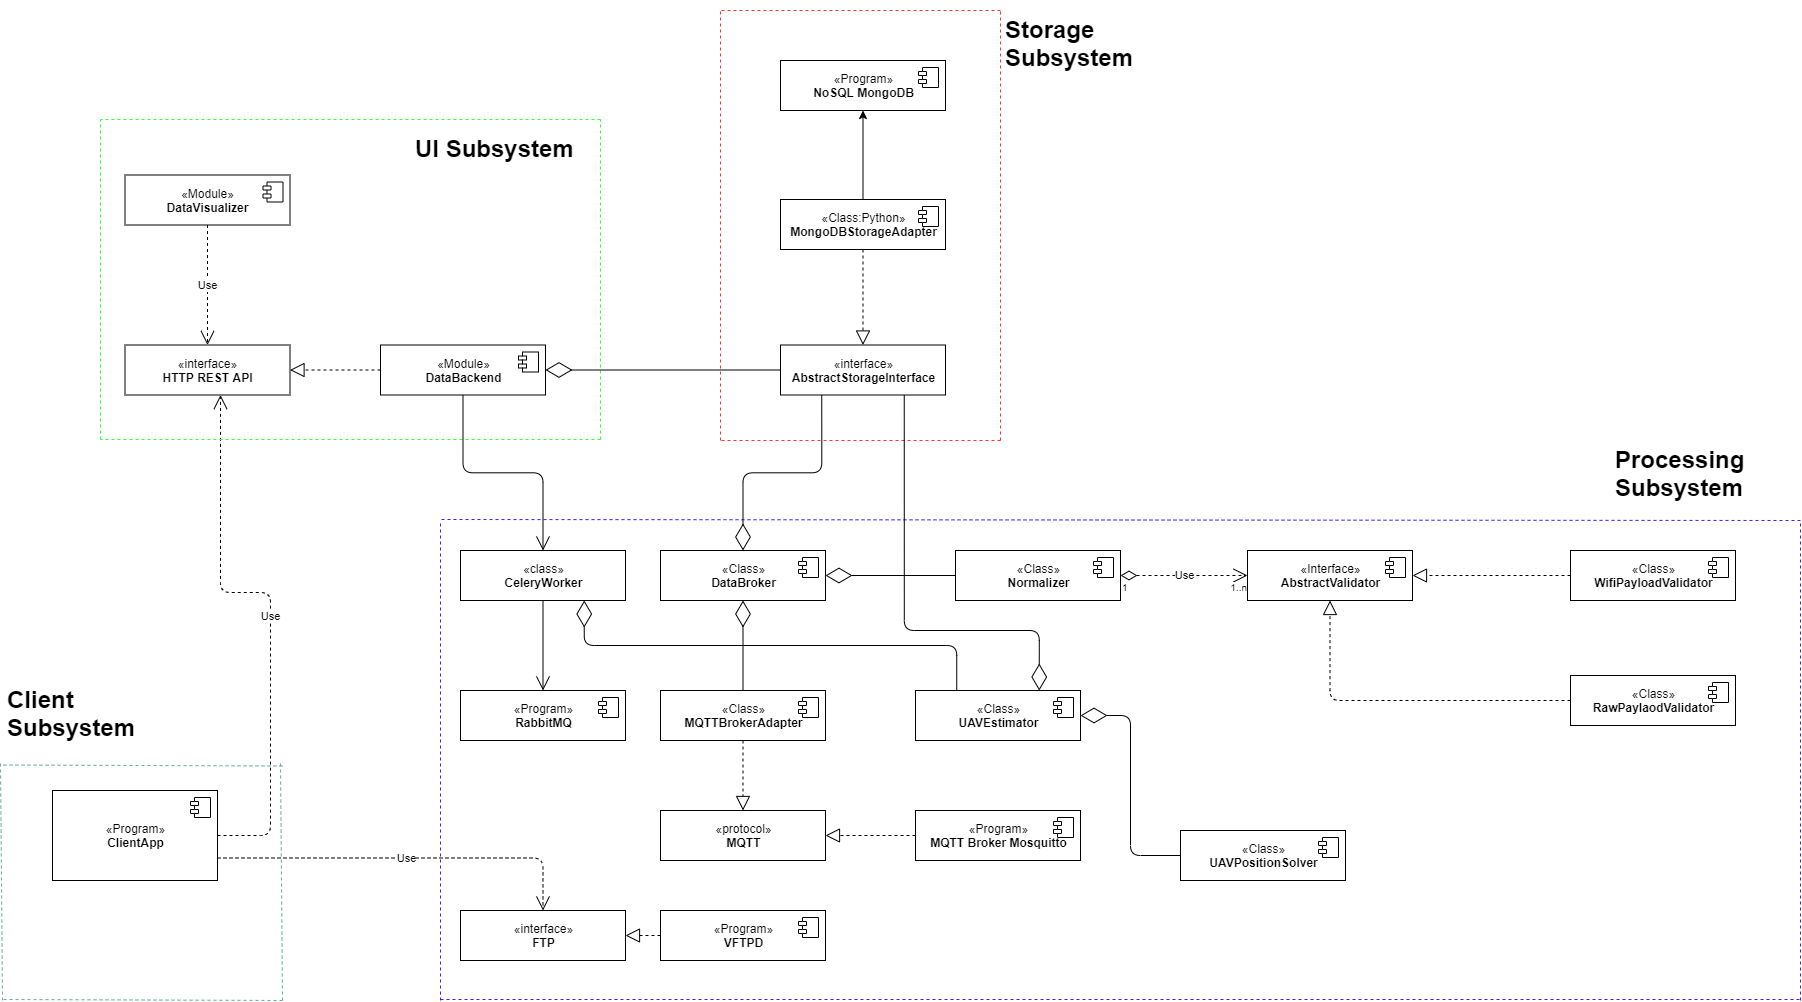
\includegraphics[width=\linewidth]{schemes/classes/ClassDiagram_overview.png}
\caption{Level 1 Main scope}
\end{figure}

\subsubsection{Motivation}\label{motivation}

The main motivation of this structure is the flexibility gaining by
dividing the responsibility of implementation. Since the project is not
so difficult, it involves a lot of different technologies and
participants.

\subsubsection{Component consideration}\label{component-consideration}

The framework highly utilize already completed components and protocols.
The most important off-the-shelf components here are:

\begin{enumerate}
\def\labelenumi{\arabic{enumi}.}
\tightlist
\item
  Interfaces

  \begin{itemize}
  \item
    \textbf{AbstractStorageAdapter} - specify methods of accessing the
    data in a strict format.
  \item
    \textbf{AbstractValidator} - defines methods to check if a message
    has a valid telemetry data format.
  \item
    \textbf{HTTP REST API} - defines methods on how to access the stored
    data through HTTP requests.
  \end{itemize}
\item
  Protocols

  \begin{itemize}
  \item
    \textbf{FTP} - used to measure uplink/downlink throughput.
  \item
    \textbf{MQTT} - used to communicate the telemetry messages to the
    MQTT Broker.
  \end{itemize}
\item
  Program

  \begin{itemize}
  \item
    FTP-server - VSFTPd - implementation of FTP server.
  \item
    MQTT Broker - Eclipse Mosquitto - implementation of MQTT Protocol
    Broker.
  \item
    NoSQL Database - MongoDB - a NoSQL database to store messages in
    BSON format.
  \item
    Queue Broker - RabbitMQ - a message queue used to register the users
    scheduled tasks.
  \end{itemize}
\end{enumerate}

\subsection{Level 2. Subsystems}\label{level-2.-subsystems}

\subsubsection{Processing Subsystem}\label{processing-subsystem}

\begin{figure}[!h]
	\centering
	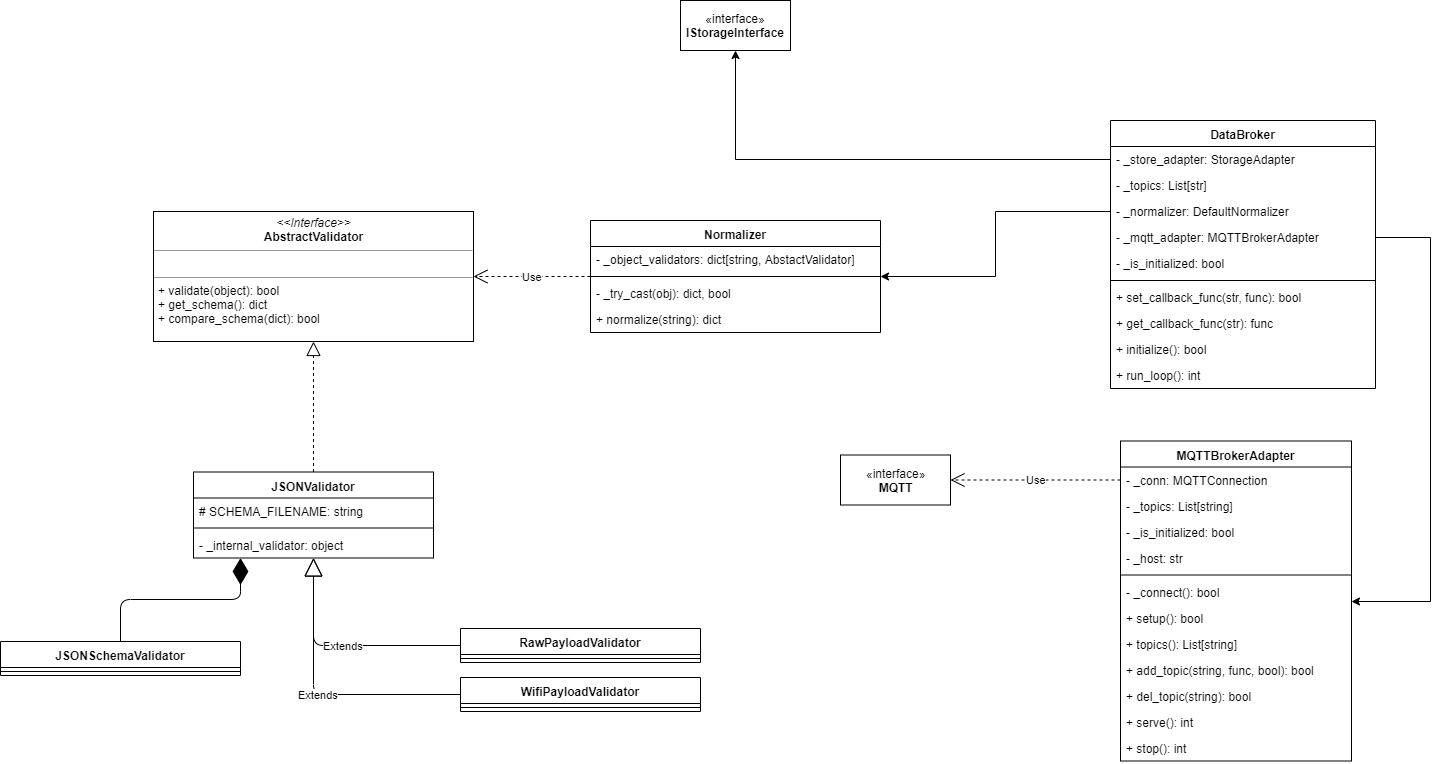
\includegraphics[width=\linewidth]{schemes/classes/ClassDiagram-processing_subsystem.png}
\caption{Processing Subsystem}
\end{figure}

\paragraph{Description}\label{description}

\textbf{Processing Subsystem} includes all functions to receive,
prepare, transform, analyze and save the data. From the conceptual
design phase it includes the following components:

\begin{itemize}
\item
  Analyzer
\item
  MessageBroker
\item
  DataBroker (deprecated, use direct pushing to DataBackend via HTTP)
\end{itemize}

These components currently implemented in Python. Some code regarding
placement optimization algorithms are private and provided to the
production environment as installation packages of code written in
Python as well.

\paragraph{Open Issues}\label{open-issues}

\subparagraph{MQTT Broker doesn't hold message for the
future}\label{mqtt-broker-doesnt-hold-message-for-the-future}

Since we use quite simple MQTT protocol, the used implementation of MQTT
Eclipse Mosquitto doesn't hold messages if here no subscribers for that
message's topic. It requires at least one subscriber or set up properly
QoS to guarantee that the message will be delivered and consumed
properly.

One of the possibilities is to use more advanced publisher/subscriber
systems such as Apache Kafka, but that has its drawbacks.

\subsubsection{Storage Subsystem}\label{storage-subsystem}

\begin{figure}[H]
	\centering
	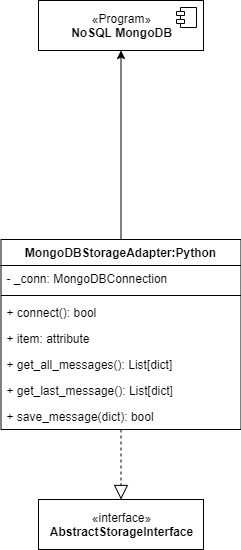
\includegraphics[width=\linewidth,height=0.4\textheight,keepaspectratio]{schemes/classes/ClassDiagram-storage_subsystem.png}
\caption{Storage Subsystem}
\end{figure}

\paragraph{Description}\label{description-1}

\textbf{Storage Subsystem} implements the function to access the stored
data. It hides all complexity and preparation phases to get the
information in the required form. This is the \textbf{Storage} component
from the conceptual design phase.

Currently, only MongoDB is supported as final storage.

The MongoDB adapter is available only in Python currently.

\subsubsection{User Interface
Subsystem}\label{user-interface-subsystem}

\begin{figure}[!h]
	\centering
	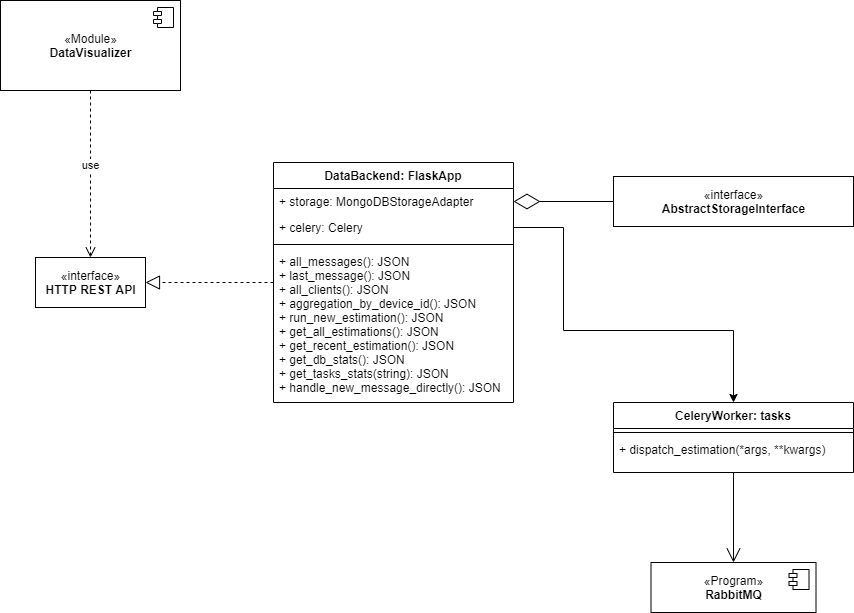
\includegraphics[width=\linewidth, keepaspectratio]{schemes/classes/ClassDiagram-ui_subsystem.png}
\caption{UI Subsystem}
\end{figure}

\paragraph{Description}\label{description-2}

The DataBackend is written in Python. It has access to the Celery Worker
infrastructure that requires RabbitMQ. This is needed to properly
register the task by the user, so it quite tangled.

The tasks performed in the background so feedback of the web backend
server is quite fast. The users can check the task status through REST
API (not implemented, //TODO).

This subsystem includes the components from the conceptual design phase:

\begin{itemize}
\item
  DataBackend
\item
  DataVisualizer
\end{itemize}

The DataVisualizer is implemented as a web Single Page Application
written with web technologies.

\subsubsection{Client Subsystem}\label{client-subsystem}

\begin{figure}[!h]
	\centering
	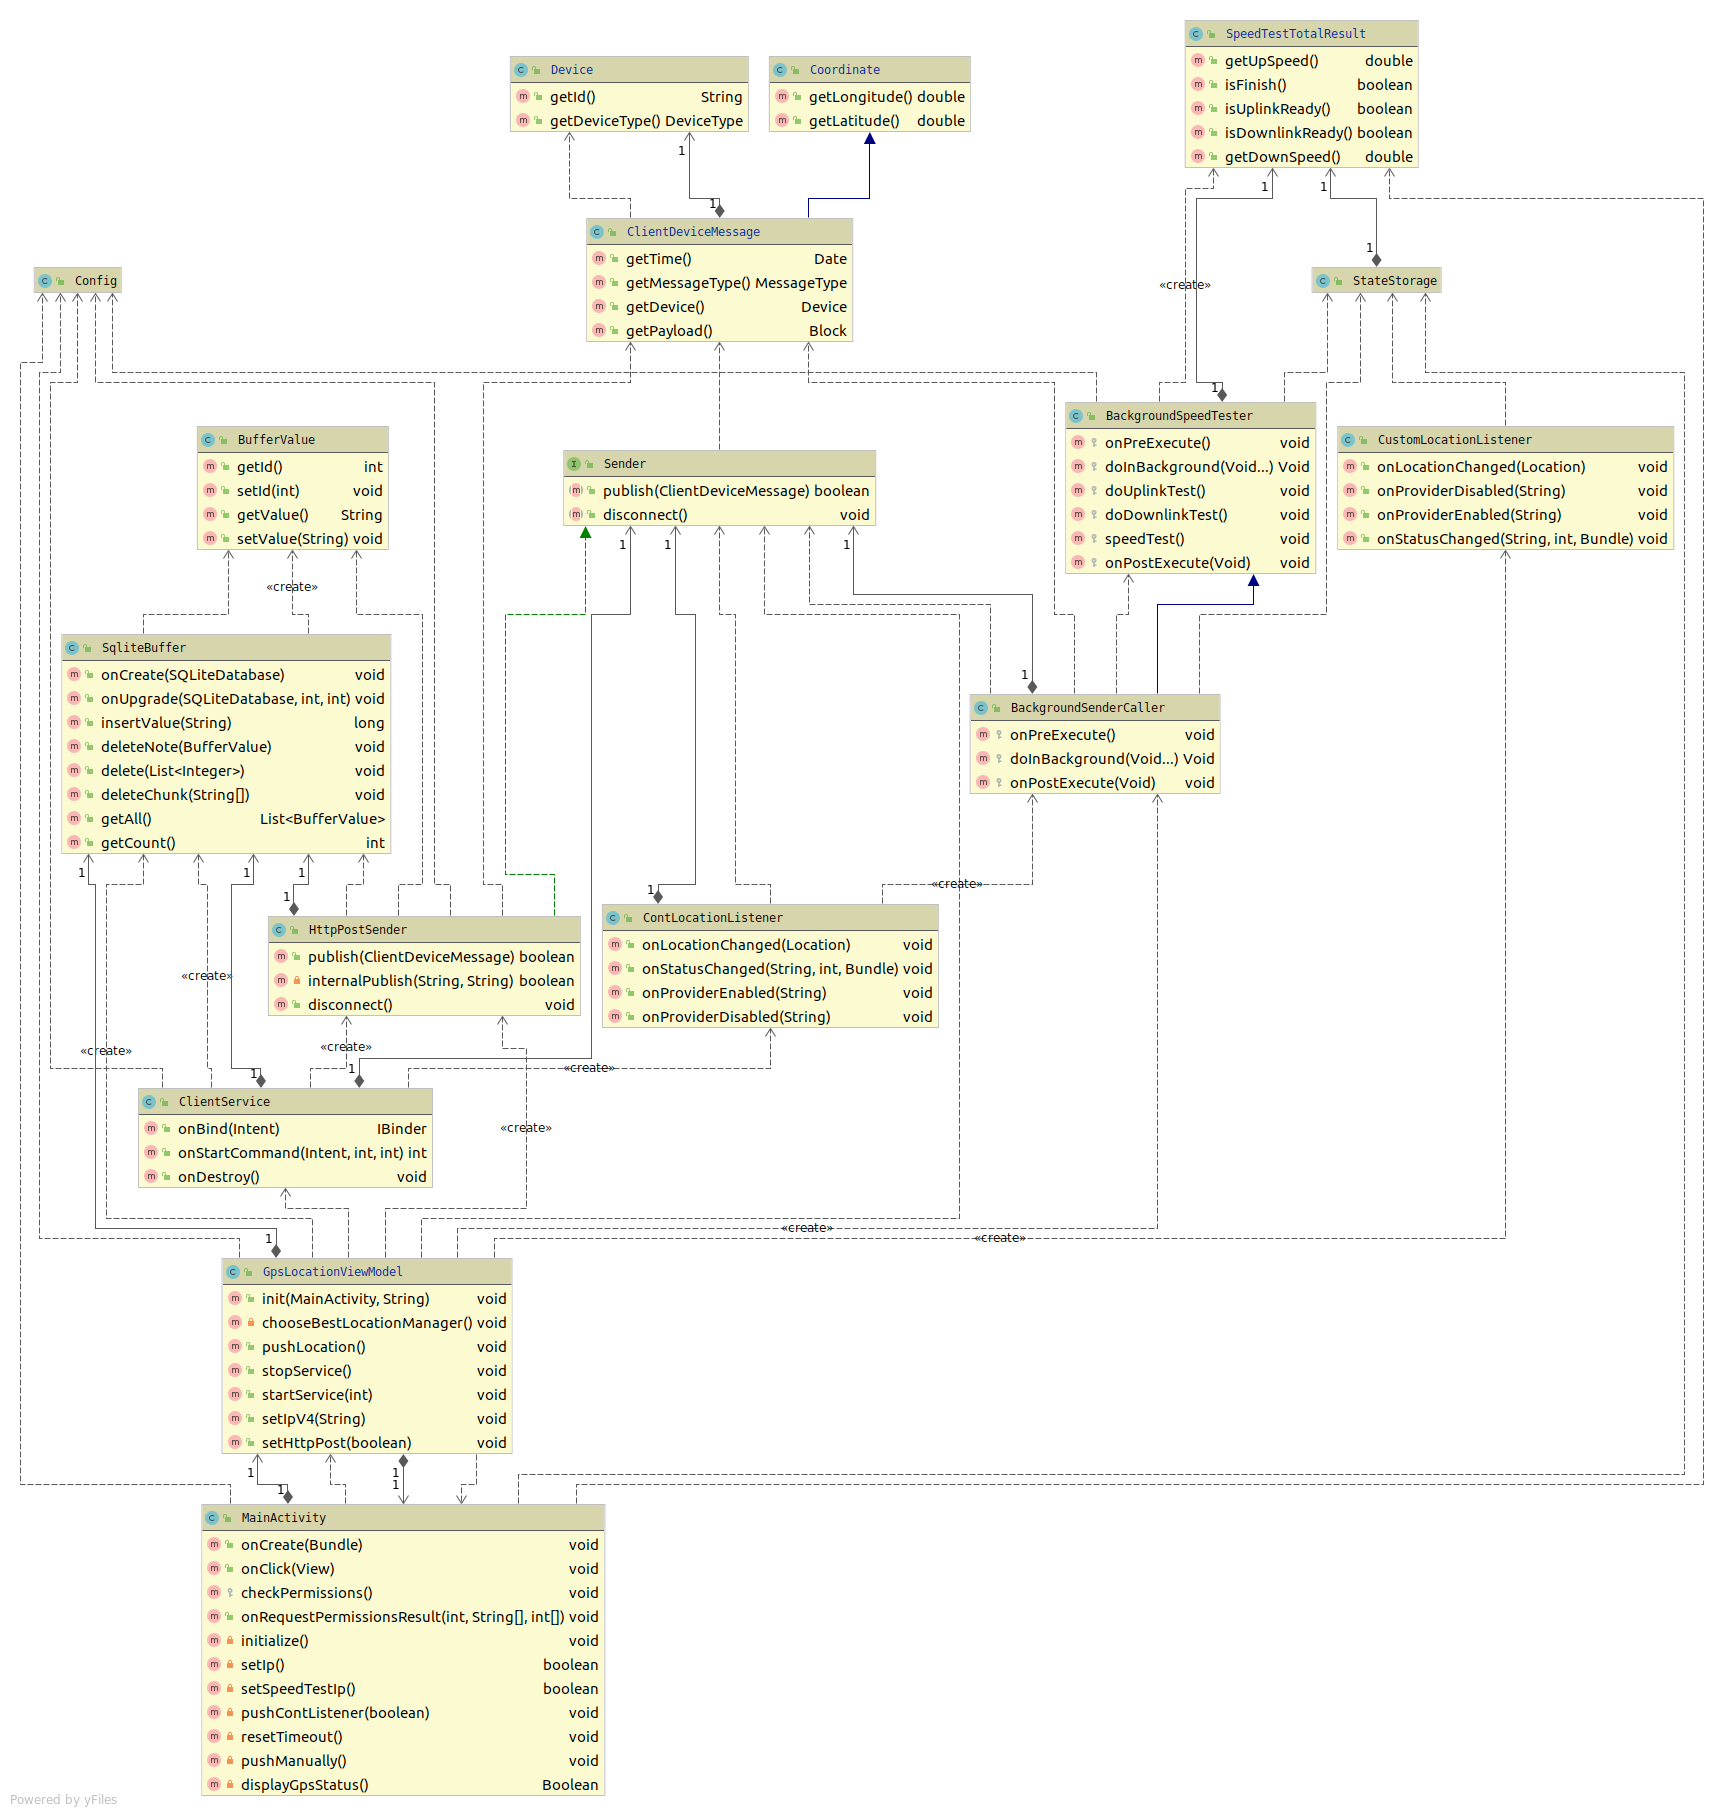
\includegraphics[width=\linewidth]{schemes/classes/android/class.png}
\caption{AndroidOverview}
\end{figure}

Android application implements MVVM architecture pattern and contains
classes to collect, store and send data about location and wifi
connection.

\begin{longtable}[]{@{}ll@{}}
\toprule
\begin{minipage}[b]{0.3\columnwidth}\raggedright
Component\strut
\end{minipage} & \begin{minipage}[b]{0.6\columnwidth}\raggedright
Description\strut
\end{minipage}\tabularnewline
\midrule
\endhead
\begin{minipage}[t]{0.3\columnwidth}\raggedright
MainActivity\strut
\end{minipage} & \begin{minipage}[t]{0.6\columnwidth}\raggedright
Application entry point. This class contains data which will be
initialize when application is started. \texttt{onCreate} method create
view using \texttt{initialization()}, check permission using
\texttt{checkPermissions()}, add handlers for every button and input
field.\strut
\end{minipage}\tabularnewline
\begin{minipage}[t]{0.3\columnwidth}\raggedright
GpsLocationViewModel\strut
\end{minipage} & \begin{minipage}[t]{0.6\columnwidth}\raggedright
Class for init and store location manager, creating background services
using \texttt{startService}, call data sender and connection quality
measurement tasks\strut
\end{minipage}\tabularnewline
\begin{minipage}[t]{0.3\columnwidth}\raggedright
StateStorage\strut
\end{minipage} & \begin{minipage}[t]{0.6\columnwidth}\raggedright
Storage to store last knowing location and speed test results.
\texttt{MainActivity} listen to this class and update data on User
Interface if data was changed\strut
\end{minipage}\tabularnewline
\begin{minipage}[t]{0.3\columnwidth}\raggedright
Config\strut
\end{minipage} & \begin{minipage}[t]{0.6\columnwidth}\raggedright
Class to store project configuration, such as sender configuration,
timeout, min location change handling and etc.\strut
\end{minipage}\tabularnewline
\begin{minipage}[t]{0.3\columnwidth}\raggedright
ClientService\strut
\end{minipage} & \begin{minipage}[t]{0.6\columnwidth}\raggedright
Background service which retrieve connection quality and send it with
given periodicity\strut
\end{minipage}\tabularnewline
\begin{minipage}[t]{0.3\columnwidth}\raggedright
SqliteBuffer\strut
\end{minipage} & \begin{minipage}[t]{0.6\columnwidth}\raggedright
Sqlite data storage for messages, which were not send to selected server
due to connection error\strut
\end{minipage}\tabularnewline
\begin{minipage}[t]{0.3\columnwidth}\raggedright
BufferValue\strut
\end{minipage} & \begin{minipage}[t]{0.6\columnwidth}\raggedright
Data Model for Sqlite buffer storage, which contains uniq id and message
for sending\strut
\end{minipage}\tabularnewline
\begin{minipage}[t]{0.3\columnwidth}\raggedright
Sender\strut
\end{minipage} & \begin{minipage}[t]{0.6\columnwidth}\raggedright
Interface for send client connection quality information using
\texttt{publish()} method\strut
\end{minipage}\tabularnewline
\begin{minipage}[t]{0.3\columnwidth}\raggedright
HttpPostSender\strut
\end{minipage} & \begin{minipage}[t]{0.6\columnwidth}\raggedright
Sender http connection implementation using post method. If connection
is not reachable, all data is stored in \texttt{SqliteBuffer}\strut
\end{minipage}\tabularnewline
\begin{minipage}[t]{0.3\columnwidth}\raggedright
ContLocationListener\strut
\end{minipage} & \begin{minipage}[t]{0.6\columnwidth}\raggedright
Listener for background ClientService, this class listen location
changes with the given period and call background task to send data
using given \texttt{Sender}\strut
\end{minipage}\tabularnewline
\begin{minipage}[t]{0.3\columnwidth}\raggedright
CustomLocationListener\strut
\end{minipage} & \begin{minipage}[t]{0.6\columnwidth}\raggedright
Listener for send data manually using \texttt{push\ manually} button on
User Interface, This listener update last knowing location in
\texttt{StateStorage}\strut
\end{minipage}\tabularnewline
\begin{minipage}[t]{0.3\columnwidth}\raggedright
BackgroundSpeedTester\strut
\end{minipage} & \begin{minipage}[t]{0.6\columnwidth}\raggedright
Task to make background uplink and downlink speed tests for wifi
connection using given server ip\strut
\end{minipage}\tabularnewline
\begin{minipage}[t]{0.3\columnwidth}\raggedright
BackgroundSenderCaller\strut
\end{minipage} & \begin{minipage}[t]{0.6\columnwidth}\raggedright
Background task for sending data\strut
\end{minipage}\tabularnewline
\begin{minipage}[t]{0.3\columnwidth}\raggedright
SpeedTestTotalResult\strut
\end{minipage} & \begin{minipage}[t]{0.6\columnwidth}\raggedright
Data model, which contain uplink and dowlink test results\strut
\end{minipage}\tabularnewline
\begin{minipage}[t]{0.3\columnwidth}\raggedright
Device\strut
\end{minipage} & \begin{minipage}[t]{0.6\columnwidth}\raggedright
Data model, which contains information about device\strut
\end{minipage}\tabularnewline
\begin{minipage}[t]{0.3\columnwidth}\raggedright
Coordinate\strut
\end{minipage} & \begin{minipage}[t]{0.6\columnwidth}\raggedright
Data model, which contains coordinates\strut
\end{minipage}\tabularnewline
\begin{minipage}[t]{0.3\columnwidth}\raggedright
ClientDeviceMessage\strut
\end{minipage} & \begin{minipage}[t]{0.6\columnwidth}\raggedright
Data model, which contains information about device, coordination and
connection quality\strut
\end{minipage}\tabularnewline
\bottomrule
\end{longtable}
